\xiti
\begin{xiaotis}

\xiaoti{在梯形 $ABCD$ 中, 已知 $AB \pingxing BC$, $AD = AB$, $BC = BD$, $\angle A = 120^\circ$, 求其他三个角的度数。}

\xiaoti{已知直角梯形的一腰长 $10\;\limi$, 这条腰和一个底所成的角是 $30^\circ$, 求另一条腰的长。}

\xiaoti{梯形的上底长为 $4\;\limi$, 过它的一个端点引一腰的平行线与下底相交, 所得三角形的周长是 $12\;\limi$。 求这个梯形的周长。}

\xiaoti{}%
\begin{xiaoxiaotis}%
    \xxt[\xxtsep]{已知:梯形 $ABCD$ 中,$AD \pingxing BC$, $DC > AB$, $BC > AD$。 求证:$\angle B > \angle C$。}

    \xxt{已知: 梯形 $ABCD$ 中,$AD \pingxing BC$, $\angle B > \angle C$, $BC > AD$。 求证: $DC > AB$。}

\end{xiaoxiaotis}

\xiaoti{画梯形 $ABCD$, 使底 $AD = 3\;\limi$, $BC = 6\;\limi$, 腰 $AB = 4\;\limi$, $\angle B = 60^\circ$。}

\xiaoti{按下图,用两种不同的方法证明等腰梯形的判定定理。}

\begin{figure}[htbp]
    \centering
    \begin{minipage}[b]{9.5cm}
        \centering
        \begin{tikzpicture}
    \begin{scope}
        \tkzDefPoints{0/0/B, 3/0/C, 0.8/1.5/A, 2.2/1.5/D}
        \tkzDrawPolygon(A,B,C,D)
        \tkzLabelPoints[left](A,B)
        \tkzLabelPoints[right](D,C)

        \tkzDefLine[parallel=through A](D,C)  \tkzGetPoint{e}
        \tkzInterLL(A,e)(B,C)  \tkzGetPoint{E}
        \tkzDrawSegment[dashed](A,E)
        \tkzLabelPoints[below](E)
    \end{scope}

    \begin{scope}[xshift=5cm]
        \tkzDefPoints{0/0/B, 3/0/C, 0.8/1.5/A, 2.2/1.5/D}
        \tkzDrawPolygon(A,B,C,D)
        \tkzLabelPoints[left](A,B)
        \tkzLabelPoints[right](D,C)

        \tkzDefLine[altitude](B,A,C)  \tkzGetPoint{E}
        \tkzDefLine[altitude](B,D,C)  \tkzGetPoint{F}
        \tkzDrawSegments[dashed](A,E  D,F)
        \tkzMarkRightAngle(A,E,B)
        \tkzMarkRightAngle(D,F,C)
        \tkzLabelPoints[below](E,F)
    \end{scope}
\end{tikzpicture}


        \caption*{(第 6 题)}
    \end{minipage}
    \qquad
    \begin{minipage}[b]{5cm}
        \centering
        \begin{tikzpicture}
    \pgfmathsetmacro{\a}{3}
    \pgfmathsetmacro{\b}{2.5}
    \pgfmathsetmacro{\c}{4}

    \tkzDefPoints{0/0/c1, \c/0/c2, 0/0.8/b1, \b/0.8/b2, 0/1.6/a1, \a/1.6/a2}
    \tkzDrawSegments[xianduan={below=0pt}](a1,a2  b1,b2  c1,c2)
    \tkzLabelSegment[above](a1,a2){$a$}
    \tkzLabelSegment[above](b1,b2){$b$}
    \tkzLabelSegment[above](c1,c2){$c$}
\end{tikzpicture}


        \caption*{(第 8 题)}
    \end{minipage}
\end{figure}

\xiaoti{已知等腰梯形的锐角等于 $60^\circ$, 它的两底分别为 $15\;\limi$, $49\;\limi$。 求它的腰长。}

\xiaoti{作等腰梯形,使高为 $a$, 上底为 $b$, 下底为 $c$。}

\end{xiaotis}

